\chapter{Weighted Fitted Q-Iteration}
  \vspace{2cm}

  \lettrine[lines=2]{I}n this chapter we introduce the central algorithm of this thesis: Weighted Fitted Q-Iteration (from now on abbreviated as WFQI from now on).\newline
  The WFQI algorithm is a \textit{batch-mode} reinforcement learning algorithm which, as the FQI algorithm described in Chapter 2, try to build
  an approximation of the Q-function of the MDP by iteratively extending the optimization horizon.\newline
  WFQI is built on top of FQI, it maintains all the properties described in the previous chapters but it also uses
  the additional information in the dataset to permit the transfer of experience sample.\newline
  Again it is a batch-mode learning algorithm so the learning procedure is divided into two distinct parts: in the first part
  samples are collected, according to some policy, only from the target task. In the second part the samples in the dataset
  are actually used to approximate the Q-function.\newline
  One important difference with respect to the standard FQI algorithm consists in the information required: each sample
  must contain additional information to permit its transfer. The overall transfer procedure, in conjunction with
  importance sampling, is depicted in figure \ref{transferwfqi}.

  \noindent Another important property, inherited from FQI, is the use of a regression algorithm in the learning phase of the algorithm
  Again this simple idea permits WFQI to take advantage of the specific regression algorithm.
  Moreover our \textit{weighed} approach to the problem of transfer, being it totally separate from weight calculation procedure,
  permits a very high flexibility in the transfer process. Ideally, we could select the weights that perfectly minimizes the effect
  of the negative transfer. In general, depending on the specific problem, many others choices are possible.\newline

  \noindent A key point in our approach is the use of weights along with the samples in the datasets. These weights
  are defined according to idea behind \textit{importance sampling}.\newline
  In many applications, we face the problem of estimating the mean of a random variable $\mu = \mathrm{E}[f(\pmb{X})]$
  where the function $f(x)$ is always 0 except for a small region $R$ and the probability for $\pmb{X}$ to
  assumes values in $R$, $\mathbb{P}(\pmb{X} \in R)$, is very small.\newline
  In such situation the application of stochastic methods, like Monte Carlo, fails because it is very difficult to have
  even one point inside the interesting region $R$. Problems of this type arise very often in practice and in very
  different domains such as physics, bayesian inference, rare events simulations etc.\newline
  The central point is that to effectively apply Monte Carlo-like techniques some points from the interesting (important)
  region must somehow be taken. The idea of importance sampling is to take samples not from the original distribution
  of $\pmb{X}$ but from an auxiliary distribution, known as the \textit{importance distribution}, that overweights the important
  region, hence the name \textit{importance} sampling.\newline
  \noindent The use of importance sampling can bring huge gains and make tractable problems where Monte Carlo is
  usually ineffective. On the other hand there are also known situation where the use of an importance distribution
  in place of the nominal one can be a disadvantage yielding estimates with extremely high variance (in some case infinite).\newline

  \noindent The first part of this chapter is dedicated to the description and motivation of WFQI, while the remaining is
  devoted to the problem of the weights estimation.

  \vspace{3cm}
  \section{The WFQI Algorithm}
    \noindent In this section we describe WFQI and we analyze its properties and relationship with respect to FQI.
    Notice that, being the weight estimation problem totally separated from WFQI, in this section we describe
    WFQI assuming that the weights for each sample are known.

    \begin{figure}
      \centering
      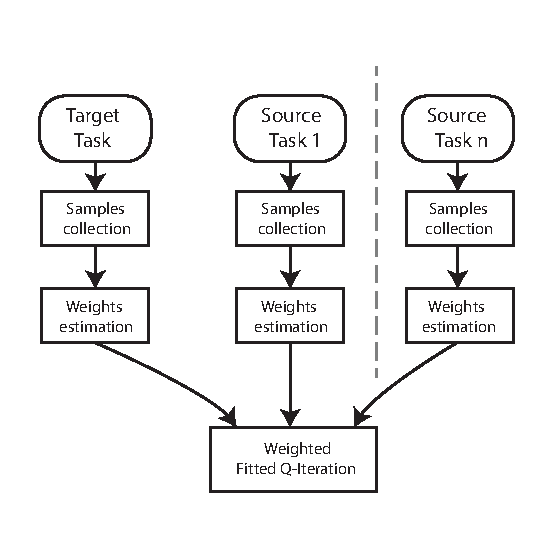
\includegraphics[scale=1.2]{images/transferwfqi.pdf}
      \caption{The overall process of transfer: from the collection to the use with WFQI}
      \label{transferwfqi}
    \end{figure}
    \noindent Algorithm \ref{fittedqw} describes a pseudocode version of Weighted Fitted Q-Iteration.

    \begin{algorithm}[H]
        \caption{Weighted Fitted Q-Iteration algorithm}\label{fittedqw}
        \begin{algorithmic}[1]
          \Procedure{WFQI($\mathcal{D} = (s,a,s',r,w_s,w_r)_{k=1}^{N}, myWeightedRegressionAlg$)}{}
            \State $k \gets 0$
            \State $\hat{Q}^{0}(s,a) \gets 0$ $\forall (s,a) \in S \times A$
            \State $D' \gets (s_k,a_k,r_k)_{k=1}^{N}$
            \State $\hat{Q}^{1} \gets myWeightedRegressionAlg(\mathcal{D}', w_r)$

            \State $\mathcal{D}' = \emptyset$
            \While {$checkStoppingCriteria()$}
              \State $k \gets k + 1$
              \For {$l = 1$ $\text{to}$ $N$}
                \State $i_l = (s_l, a_l)$
                \State $o_l = Q^{1} + \gamma \max_{a' \in A} \hat{Q}_{k-1}(s',a')$
                \State $\mathcal{D}' \text{+=}$ $(i_l,o_l)$
              \EndFor
              \State $\hat{Q}^{k} \gets myWeightedRegressionAlg(\mathcal{D}', w_s)$
            \EndWhile
          \EndProcedure
        \end{algorithmic}
    \end{algorithm}

    \noindent More informations about the specific implementation of WFQI are given in appendix A.\newline

    \noindent The main differences with respect to the standard FQI algorithm are:
    \begin{itemize}
      \item \textbf{Dataset}: The experience sample contained in the dataset are enhanced with additional
        information namely $w_r$ and $w_s$. These informations are needed by WFQI in order to permit
        the transfer of samples coming from different source tasks. These weights, for reward ($w_r$) and
        transition model ($w_p$), need to be separately estimated and then injected inside the
        existing dataset.

      \item \textbf{Regression Algorithm}: The only real modification needed in algorithm \ref{fittedqw},
        with respect to the standard FQI, consists in a new requirement over the used
        regression algorithm: in order to effective transfer samples, the regression
        algorithm must permit to specify, for each sample, a weight and accordingly use
        it in the fitting procedure. Notice that different weights are used in different
        part of the algorithm; at the iteration 0 the Q-function is initialized to zero
        this means that the initial dataset is exclusively built using the rewards of the
        sample thus making useless the use of $w_s$. Moreover, in the successive iterations,
        instead of building the dataset $\mathcal{D}'$ using the usual Bellman equation
        $o_l = r + \gamma \max_{a' \in A} \hat{Q}^{k-1}(s',a')$ we substitute $r$ with $\hat{Q}^{1}$
        which represents the weighted reward function (according to $w_r$), thus, in the regression
        we only need to weight the samples with $w_s$.
    \end{itemize}

  \section{Algorithm Motivation}
    \noindent The motivation of using Importance Sampling in the framework of Transfer Learning comes directly
    from the need of a strong theoretical basis behind the transfer procedure. Many sample-based transfer approaches,
    see for example \cite{lazaric2008transfer}, focus on defining measures to capture the concept of similarity
    between tasks and samples. In our case, the possibility to support the calculation and use of each weight
    with a strong theoretical background gives the possibility, not only to perform an effective transfer of samples,
    but also to quantify and control the amount of bias introduced in the estimation.\newline

    \noindent WFQI exploits the same idea of the standard FQI algorithm. It uses a dataset of experience
    sample, previously collected, in conjunction with a generic weighted regression algorithm to produce an estimation
    of the Q-function for the target task. The main difference, as already outlined above, is that it permits
    the use of samples coming from tasks different from the one it tries to solve.\newline
    If we assume that $w_p$, $w_r$ are the \textit{ideal} weights (ie. given by an oracle),
    then, according to the results of importance sampling presented in the previous chapter, the use of
    the corresponding samples coming from the set of source tasks is unbiased and may lead to a potential
    reduction in the variance of the estimation.\newline
    On the other side, the ideal weights can not be calculated in practice given that their knowledge would
    require a perfect knowledge of the reward and transition model of the target task meaning that nothing has to
    be learned. When using the estimated weights the use of the corresponding samples from the set of source tasks in
    the learning process of the target is not unbiased. This means that in addition to the potential reduction in
    variance an additional increase in bias is possible.\newline
    The necessity of calculating the pair of weights for each source sample motivates the need of explicitly modelling
    the reward and transition model for all the tasks involved in the transfer (this problem will be addressed in the
    final part of this chapter).

    \noindent Another important characteristic of WFQI is the peculiar use of the weights associated with each
    samples, that permits to transfer samples even in situations where either the reward or the dynamics
    represented by the sample is significantly different from the target task.
    \noindent A formal and detailed theoretical analysis of the errors coming from the use of estimated weights
    is provided in the last sections of this Chapter.\newline

    \noindent In conclusion WFQI represents a very simple and intuitive modification of
    the original FQI algorithm. Besides, these adjustments do not negatively affect the computational
    complexity of the algorithm (only two additional multiplication per iteration are needed) and
    has the remarkable advantage of permitting the reuse of past knowledge (which in general tends to speed-up the learning process).\newline
    It also important to note some of the possible disadvantages: WFQI uses extensively the underlying idea
    of importance sampling and therefore may not be effective in every situation.

\section{Introduction to Importance Sampling}
  \noindent In this section, and in the remaining part of this Chapter, we introduce the general theory of Importance Sampling (sometimes abbreviated as IS), we start from a problem apparently
  unrelated with the problem of transfer in RL, later we describe how the transfer of samples across tasks can be reframed into
  the general idea of IS.\newline

  \noindent Let $\pmb{X}$ be a continuous random variable distributed according to a density function $p(x)$. Our problem is to find:
  \begin{equation}
    \mu = \mathrm{E}[f(\pmb{X})] = \int_{\mathcal{R}} f(\pmb{x})p(\pmb{x}) d\pmb{x}
    \label{mean1}
  \end{equation}
  \noindent where $p$ is a probability density function over $\mathcal{R} \subseteq \mathbb{R}^{d}$ and $f$ is a
  generic function over $\pmb{X}$. $p$ is known as the \textbf{nominal distribution}.\newline
  As already stated we want to estimate the mean of $f(\pmb{X})$ not from samples drawn from $p$ but from a set
  of samples drawn from an auxiliary distribution $q$ from now on known as the \textbf{importance distribution}.
  Recalling equation \ref{mean1} we have with simple algebraic manipulation:
  \begin{equation*}
    \mu = \int_{\mathcal{R}} f(\pmb{x})p(\pmb{x}) d\pmb{x} = \int_{\mathcal{R}} f(\pmb{x}) \frac{p(\pmb{x}) q(\pmb{x})}{q(\pmb{x})} d\pmb{x} =
     \mathbb{E}_{q} \left [f(\pmb{X})\frac{p(\pmb{X})}{q(\pmb{X})} \right ]
  \end{equation*}
  $w(\pmb{x}) = \frac{p(\pmb{x})}{q(\pmb{x})}$ is the \textbf{importance weight} for the sample $\pmb{x}$. The result
  is very intuitive: we can estimate the mean of $f(\pmb{X})$ by drawing samples from $q$ and correcting them
  with a multiplicative factor equal to $\frac{p(\pmb{X})}{q(\pmb{X})}$.\newline

  \noindent Notice that the probability density function $q(x)$ does not to be strictly positive everywhere but it sufficient
  to have $q(x) > 0$ whenever $f(x)p(x) \neq 0$. It is also important to notice that $q(x)$ can never be equal to 0
  (if a sample has been drawn from $q$ then $q(x) > 0$ in any case).\newline

  \noindent We now proceed to give some additional definition and we state some results to understand when the use of importance sampling
  is useful and when it is not.\newline
  We define the importance sampling \textit{estimate}, $\hat{\mu}_q$, of $\mu$ as
  \begin{equation}
    \hat{\mu}_q = \frac{1}{N} \sum_{i=1}^{N} \frac{f(X_i)p(X_i)}{q(X_i)}
    \label{meanestimate}
  \end{equation}

  \noindent The fundamental point is that we are able to compute the estimate in \ref{meanestimate} only when both $p$ and $q$ are known.
  This is not always the case, in particular when we will try to apply these ideas to the problem of the transfer of knowledge
  we will need to resort to some method to estimate the ration between the two densities. For this section we will assume that
  the ration $p/q$ is computable.

  \begin{theorem}[\cite{importance2013Owen}]
    Let $\hat{\mu}_q$ the estimate provided by equation \ref{meanestimate} where $\mu = \int_{\mathcal{D}} f(\pmb{x})p(\pmb{x}) d\pmb{x}$
    and $q(\pmb{x}) > 0$ whenever $f(\pmb{x})p(\pmb{x}) \neq 0$. Then $\mathbb{E}_{q}[\hat{\mu}_q] = \mu$ and $\text{Var}_{q}[\hat{\mu}_q] = \frac{\sigma^{2}_{q}}{N}$
    where
    \begin{equation}
       \sigma^{2}_{q} = \int_{\mathcal{D}} \frac{(f(\pmb{x}) p(\pmb{x}))^2}{q(\pmb{x})} d\pmb{x} - \mu^{2} = \int_{\mathcal{D}} \frac{(f(\pmb{x}) p(\pmb{x}) - \mu q(\pmb{x}))^{2}}{q(\pmb{x})} d\pmb{x}
       \label{theorem2}
    \end{equation}
  \end{theorem}
  \begin{proof}
    Let $\mathcal{Q} = \{\pmb{x} | q(\pmb{x}) > 0\}$ then
    \begin{equation*}
      \begin{multlined}
        \mathbb{E}_{q} \left [ \frac{f(\pmb{X})p(\pmb{X})}{q(\pmb{X})} \right ] = \int_{\mathcal{Q}} \frac{f(\pmb{x})p(\pmb{x})}{q(\pmb{x})} q(\pmb{x}) d\pmb{x} = \int_{\mathcal{Q}} f(\pmb{x}) p(\pmb{x}) d\pmb{x} = \\
        \int_{\mathcal{D}} f(\pmb{x}) p(\pmb{x}) d\pmb{x} + \int_{\mathcal{Q} \cap \mathcal{D}^{c}} f(\pmb{x}) p(\pmb{x}) d\pmb{x} - \int_{\mathcal{D} \cap \mathcal{Q}^{c}} f(\pmb{x}) p(\pmb{x}) d\pmb{x} = \\
        \int_{\mathcal{D}} f(\pmb{x}) p(\pmb{x}) d\pmb{x} = \mu = \mathbb{E}_{q}[\hat{\mu}_q]
      \end{multlined}
    \end{equation*}

    \noindent The second part of the proof can be obtained in a similar way:
    \begin{equation*}
      \text{Var}[\hat{\mu}_{q}] = \frac{1}{n} \left [ \int_{\mathcal{Q}} \left ( \frac{f(\pmb{x})p(\pmb{x})}{q(\pmb{x})} \right )^{2} q(\pmb{x}) d\pmb{x} - \mu^{2} \right ] =
        \frac{1}{n} \left [ \int_{\mathcal{D}} \left ( \frac{f(\pmb{x})p(\pmb{x})}{q(\pmb{x})} \right )^{2} q(\pmb{x}) d\pmb{x} - \mu^{2} \right ]
    \end{equation*}

    \noindent Simple manipulations gives equation \ref{theorem2}.
  \end{proof}

  \noindent Expressions in equation \ref{theorem2} give a simple way to understand when importance sampling can succeed or fail.
  The best importance distribution is the one that minimizes $\int_{\mathcal{D}} \frac{(f(\pmb{x}) p(\pmb{x}))^2}{q(\pmb{x})} d\pmb{x}$.
  Moreover if we analyze the right integral expression (always in \ref{theorem2}) it is easy to notice that the numerator is small
  when $f(\pmb{x})p(\pmb{x})$ is similar to $\mu q(\pmb{x})$. This happens when $f(\pmb{x})p(\pmb{x})$ is proportional to $q(\pmb{x})$.
  On the other hand also the denominator can cause some problems: a region with a small $q$ can amplify whatever lack of proportionality
  in the numerator.\newline
  In theory choice of $q$ such that $\sigma^{2}_{q} = 0$ are possible but of course of no use in practice. The choice
  of a good importance distribution is a complex problem that requires educated guesses, numerical search and domain-specific knowledge.


\section{Transfer with Importance Sampling}

\noindent In this section we face the problem of the transfer of knowledge across multiple tasks. We assume the context of
batch-mode reinforcement learning and, for the sake of simplicity, we suppose that a single source task is available. Later on
we will extend our transfer model for the case of multiple source tasks.\newline
We suppose some samples have been previously collected from the target task producing a dataset $\mathcal{T} = \{(s_{i},a_{i},s'_{i},r_{i})\}_{i=1}^{N_t} $ and
similarly some samples (the samples that have to be transferred) have been obtained from the source task producing a dataset $\mathcal{S} = \{(s_{i},a_{i},s'_{i},r_{i}) \}_{i=1}^{N_s}$.
Typically we will assume $N_t << N_s$.\newline

\subsection{Single Source Task}
  \noindent Suppose to transfer a sample $(s_{i}, a_{i}, s'_{i}, r_{i})$ from the source task to the target task. The transfer
  affects the target task on two sides: the reward model and the probability transition model. \newline
  Suppose, for simplicity, to consider only the effect on the reward. This last element is modeled as a function:
  \begin{equation}
    r: S \times A \rightarrow \mathbb{R}
  \end{equation}
  \noindent Given a state-action pair the function will return the expected reward for the agent. Every time a transfer
  is performed we are introducing a bias inside the estimation of the reward function for the target task.\newline
  The idea is to apply importance sampling to the samples of the source task used in the estimation of the reward function
  of the target task. Let be $w_r$ the likelihood weight associated to the reward model. Select a sample pair $(s,a,s',r)$ from
  the source task (we are assuming that the source and target share the same state-action space). Then we have
  \begin{equation}
    w_{r} = \frac{\text{likelihood of $r$ to be generated in }\mathcal{S}}{\text{likelihood of $r$ to be generate in }\mathcal{T}}
  \end{equation}

  \noindent There are some important facts to be observed:
  \begin{itemize}
    \item When the stochastic model of the reward is perfectly known in both task
      the $w_r$ can be perfectly calculated, in this setting the use of $r$ in the
      target is completely unbiased. Of course if the two tasks are quite different
      then the reduction of variance carried by $r$ will be much lower with respect to
      the case where $r$ is directly sampled from the target.

    \item In practice the reward model of the source and target tasks are not known
      (otherwise the agent has nothing to learn, at least for the reward, and transfer will
      be useless). This means that we need a procedure to accurately estimates the likelihood
      for both tasks. A possible procedure will be discussed in the next section.

    \item As already observed in the general discussion about importance sampling, the
      denominator of $w_r$ can never be zero (if the sample has been drawn from the source
      then its likelihood is by definition different from 0). Some numerical problems may arise
      when the denominator is close to zero, in such cases $w_r$ may be very large and this
      tends to increase the variance of the estimation.
  \end{itemize}

  \noindent Identical considerations hold for the probability transition model, also in this case we have
  a stochastic model that given a state-action pair returns a probability distribution over the next state.\newline
  Again the idea is to apply importance sampling also to the transition model, this means that a second
  likelihood weight $w_p$ must be defined. Fix a sample $(s,a,s',r)$ to be transferred then:
  \begin{equation}
      w_{p} = \frac{\text{likelihood of $s \rightarrow s'$ to be generated in }\mathcal{S}}{\text{likelihood of $s \rightarrow s'$ to be generate in }\mathcal{T}}
  \end{equation}

  \noindent The overall transfer procedure for the single source case requires to collect the two datasets $\mathcal{T}$ and $\mathcal{S}$ from
  the two tasks. A weight estimation procedure is applied to the datasets. The output is a new pair of datasets $\mathcal{S}'$ and $\mathcal{T}'$ where
  \begin{equation*}
    \begin{cases}
      \mathcal{S}' = \{ (s_{i},a_{i},s_{i}',r_{i},w_{r}^{i},w_{p}^{i}) \}_{i=1}^{N_s} \\
      \mathcal{T}' = \{ (s_{i},a_{i},s_{i}',r_{i},1,1) \}_{i=1}^{N_t}
    \end{cases}
  \end{equation*}
  Notice that the weights for the samples coming from the target tasks (that do not need to be transferred) are
  obviously fixed to 1.

\subsection{Multiple Source Tasks}
  \noindent The extension to the case where multiple source tasks are present is straightforward. Let $\mathcal{T}$ the dataset of the samples
  collected from the target task and let $\mathcal{S}_i$ the dataset of samples collected from the $i$-th source task.\newline
  Then the transfer procedure works exactly as in the single source case: the source datasets are considered one at a time,
  a weight estimation procedure is applied to the samples contained in the current dataset so that we obtain
  \begin{equation*}
    \mathcal{S}_{i} = \{ (s_{i}^{j}, a_{i}^{j}, s_{i}^{'j}, r_{i}^{j}, w_{r}^{i,j}, w_{p}^{i,j}) \}_{j=1}^{N_{s}}
  \end{equation*}
  This is repeated for every source tasks. As in the previous case for the target task the weights for reward and
  transition model are fixed to 1 (ie. nothing to transfer).\newline

  \noindent Two remaining open problems are:
  \begin{enumerate}
    \item How to estimates the likelihood weights for transition and reward model when the relevant densities are not known? This
    problem will be addressed in the next two sections.
    \item How to effectively use the likelihood weights inside a learning algorithm? The conclusive sections of this chapter will propose a variation
    of the well-known FQI algorithm to include the information coming from the likelihood weights.
  \end{enumerate}

\subsection{Transfer of Samples vs Transfer of Trajectories}
  \begin{figure}
    \centering
    \includegraphics{images/trajectorysample.eps}
    \caption{Trajectory vs Sample}
    \label{trajectorysample}
  \end{figure}

  \noindent One implicit assumption done so far is the type of knowledge to be transferred to the target task.
  In the last years two main approaches have been proposed: the transfer of \textit{trajectories} or the transfer
  of \textit{samples}. Figure \ref{trajectorysample} depicts the difference between the two entities.\newline
  A trajectory is characterized by an initial state, a terminal state (where the trajectory ends because either
  one of the goal state or a maximum horizon has been reached by the agent) and by a series of intermediate states
  that link the initial with the terminal state. Each state is linked with each other with an action that performs
  the transition between the two states. On the other hand, a sample is characterized by four-tuples $(s,a,s',r)$
  where $s$ is the state in which the agent is performing action $a$ reaching the successive state $s'$ and
  obtaining reward $r$.\newline

  \noindent The transfer of a sample is, in our specific transfer learning framework, more advantageous
  than the transfer of an entire trajectory. Indeed the transfer of an entire trajectory does not
  permit to decide which part of the trajectory is actually beneficial for the transfer and which are not.
  There may be part of the trajectory that could represents dynamics that may negatively bias the agent
  inside the target task.\newline
  On the other hand, the transfer of samples permits a finer control over the transfer process.
  Once the samples are collected from the source tasks we loose the information about the specific
  trajectory each sample belongs to. Our approach permits to estimate a pair of weights for each sample,
  these weights are used by the learning algorithm to correct the bias introduced by such samples.\newline

  \noindent As an example consider the problem of the transfer of a trajectory where 99 \% of the
  transition/rewards are identical as in the target task but 1 \% of the trajectory is completely
  different with respect the target the target. In this case, the overall likelihood of the trajectory
  will be approximately zero leading to an ineffective transfer. In the case we had considered each
  single sample of the trajectory a much more effective transfer could have been accomplished.

\subsection{Weights Selection}
  \noindent One key point in our transfer procedure is the calculation of the likelihood weights that are used by the
  learning to correct the negative bias. To each sample we associate a pair of weights $w_r$ and $w_p$.
  Given a sample $(s,a,s',r)$ the weight $w_r$ is defined as the ratio between the likelihood of reward $r$
  to be generated in the target task and the likelihood of $r$ to be generated in the corresponding source task
  (from which the sample has been collected). On the other side $w_p$ is the weight associated with the
  transition model and it is defined as the ratio between the likelihood for the transition $s \rightarrow s'$ to
  be generated in the target task and the likelihood, for the same transition, to generated in the correspondent source
  task.\newline

  \subsubsection{Ideal case}
    \noindent In the case where the probabilistic models for reward and transition are perfectly known it
    is possible to calculate the true values for the importance weights of each sample in the dataset.
    We assume that both reward and transition are normally distributed:
    \begin{equation}
      x_{S} \sim \mathcal{N}(\mu_{S}, \sigma^{2}), \quad x_{T} \sim \mathcal{N}(\mu_{T}, \sigma^{2})
    \end{equation}
    where $x$ is either the reward $r$ or the next state $s'$ for a sample $(s,a,x)$.\newline
    In this case the corresponding weight can be obtained applying the definition of importance weight:
    \begin{equation}
      w(x) = exp \left ( -\frac{(x-\mu_{T})^{2}}{2\sigma^{2}} \right ) exp \left ( \frac{(x-\mu_{S})^{2}}{2\sigma^{2}} \right )
      \label{ideal-weights-expr}
    \end{equation}
    Notice that we assume the variance of the reward/transition model to be identical in both the source and target task.
    This assumption is without loss of generality, indeed in the case of different variances we just need to
    consider an additional constant term, $\frac{\sigma^{2}_{S}}{\sigma^{2}_{T}}$, in Equation \ref{ideal-weights-expr}.
    This assumption will be maintained in the next chapters and sections.

  \subsubsection{Non-Ideal case}
    \noindent As already observed in the previous chapters it is not possible, in practice, to perfectly calculate
    the pair of weights for each sample in the dataset. This is due to the fact that the model for the reward and
    transitions are not known in both the source and target task. In the case they were known then we are no more
    in the settings of reinforcement learning but we are solving a dynamic programming problem where the model
    of the environment is perfectly known to the agent and the objective is to approximate the optimal policy.
    In the following, we propose a procedure to estimate the weights based on Gaussian Process (GP) regression.\newline
    The main idea behind the estimation procedure is to make a hypothesis over the reward and
    transition model. Suppose for now to consider only the estimation of the weight associated with the reward, $w_r$.
    We hypothesize a gaussian model for the reward model for both the source and target task. The idea is to place two distinct GP regressors, one for each task,
    over the entire state-action space. For an extensive discussion about GPs refer to appendix B.\newline
    Once the gaussian process has been fitted using the samples in the dataset for the source and target task, we fix
    a sample $(s,a,s',r)$ and we ask a prediction, for the pair $(s,a)$, to the GP associated with the source and to
    the GP associated with the target.\newline
    Now, we proceed to give an extensive description of the estimating procedures.

    \begin{figure}
      \centering
      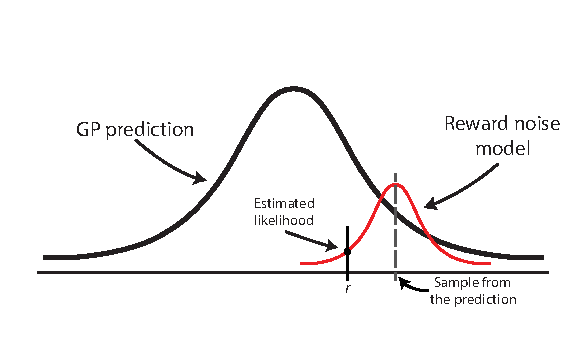
\includegraphics[scale=1.1]{images/gaussian.pdf}
      \caption{Estimating the reward/transition weight from a GP prediction.}
      \label{gaussians}
    \end{figure}

    \noindent A \textit{first} idea to obtain an estimation $\tilde{w}_{x}$ is to directly sample the weights distribution, which
    is unknown and not available in practice.\newline
    Suppose to have a source sample $(s,a,x)$, where $x$ is either $r$ or $s'$, and we want to compute
    its importance weight. First, we predict the distribution if the mean of $x$ under the target model and the
    source model using our previously fitted Gaussian Processes:
    \begin{equation}
      \tilde{\mu}_{T} \sim \mathcal{N}(\mu_{GP,T}, \sigma_{GP,T}^{2}), \quad \tilde{\mu}_{S} \sim \mathcal{N}(\mu_{GP,S}, \sigma_{GP,S}^{2})
      \label{distributions}
    \end{equation}
    Then we consider the estimated importance weights:
    \begin{equation}
      \tilde{w}(x) = \tilde{w}_{x}(\tilde{\mu}_{T}, \tilde{\mu}_{S}) = exp \left ( -\frac{(x-\tilde{\mu}_{T})^{2}}{2\sigma^{2}} \right ) exp \left ( \frac{(x-\tilde{\mu}_{S})^{2}}{2\sigma^{2}} \right )
    \end{equation}
    where the notation $\tilde{w}_{x}(\tilde{\mu}_{T})$ is used to emphasize the dependence on the two means (which now
    are random variables) and on the fixed value of $x$.\newline
    We sample $N_{smp}$ from both $\tilde{\mu}_{T}$ and $\tilde{\mu}_{S}$ then for the $i$-th sample $\mu_{x}^{i}$ we consider the
    two distributions:
    \begin{equation}
      n_{x}^{i} \sim \mathcal{N}(\mu_{x}^{i}, \sigma^{2}_{GP,T}), \quad d_{x}^{i} \sim \mathcal{N}(\mu_{x}^{i},\sigma^{2}_{GP,S})
    \end{equation}

    Then the estimation according to the $i$-th sample is given by:
    \begin{equation}
      w^{i}(x) = \frac{n^{i}(x)}{d^{i}(x)}
    \end{equation}
    Notice that when the prediction from the GP of source and target task are perfect, ie. $\sigma_{GP,T}^{2} = \sigma_{GP,S}^{2} = 0$,
    $\tilde{w}(x)$ converges to $w(x)$.
    The procedure is graphically summarized in Figure \ref{gaussians}.\newline
    Despite being a very simple approach some problems may arise when choosing the final weight among the $N_{smp}$ estimations.
    The selection of different quantiles of the weight distribution may lead, in practice, to very different performance (good in some cases, poor in others). Furthermore
    we do not have any theoretical backup to support the choice of a particular sample among the $N_{smp}$.\newline
    We are able to prove the following result on $\tilde{w}_{x}$:
    \begin{lemma}
      The expectation of $\tilde{w}_{x}(\tilde{\mu}_{T}, \tilde{\mu}_{S})$ under the distributions defined in
      Equation \ref{distributions} is:
      \begin{equation}
        \mathbb{E}[\tilde{w}_{x}(\tilde{\mu}_{T}, \tilde{\mu}_{S})] =
        \begin{cases}
          \frac{\sigma^{2}}{\sigma^{2} - \sigma^{2}_{GP,S}} \frac{\mathcal{N}(x; \mu_{GP,T}, \sigma^{2} + \sigma^{2}_{GP,T})}{\mathcal{N}(x; \mu_{GP,T}, \sigma^{2} - \sigma^{2}_{GP,S})} \quad \sigma^{2}_{GP,S} < \sigma^{2} \\
          \infty \quad Otherwise
        \end{cases}
        \label{mean-weight}
      \end{equation}
    \end{lemma}
    \begin{proof}
      Suppose that $\sigma^{2}_{GP,S} < \sigma^{2}$. Then:
      \begin{equation}
        \begin{aligned}
          & \mathbb{E}[\tilde{w}_{x}(\tilde{\mu}_{T}, \tilde{\mu}_{S})] = \iint \frac{exp \left ( -\frac{(x-\tilde{\mu}_{T})^{2}}{2\sigma^{2}} \right )}{\sqrt{2\pi\sigma^{2}}} \frac{\sqrt{2\pi\sigma^{2}}}{exp \left ( -\frac{(x-\tilde{\mu}_{S})^{2}}{2\sigma^{2}} \right )} \\
          & \frac{exp \left ( -\frac{(\tilde{\mu}_{T}-\mu_{GP,T})^{2}}{2\sigma^{2}_{GP,T}} \right )}{\sqrt{2\pi\sigma^{2}_{GP,T}}} \frac{exp \left ( -\frac{(\tilde{\mu}_{S}-\mu_{GP,S})^{2}}{2\sigma^{2}_{GP,S}} \right )}{\sqrt{2\pi\sigma^{2}_{GP,S}}} d\tilde{\mu}_{T}\tilde{\mu}_{S} \\
          & = \int \frac{exp \left ( -\frac{(x-\tilde{\mu}_{T})^{2}}{2\sigma^{2}} \right )}{\sqrt{2\pi\sigma^{2}}} \frac{exp \left ( -\frac{(\tilde{\mu}_{T}-\mu_{GP,T})^{2}}{2\sigma^{2}_{GP,T}} \right )}{\sqrt{2\pi\sigma^{2}_{GP,T}}} d\tilde{\mu}_{T} \\
          & \int \frac{\sqrt{2\pi\sigma^{2}}}{exp \left ( -\frac{(x-\tilde{\mu}_{S})^{2}}{2\sigma^{2}} \right )} \frac{exp \left ( -\frac{(\tilde{\mu}_{S}-\mu_{GP,S})^{2}}{2\sigma^{2}_{GP,S}} \right )}{\sqrt{2\pi\sigma^{2}_{GP,S}}} d\tilde{\mu}_{S}
        \end{aligned}
      \end{equation}

      \noindent The first integrand is over the product of two Gaussian densities, which is known to be (see \cite{bromiley2003products}):
      \begin{equation}
        \mathcal{N}(\tilde{\mu}_{T}; \bar{\mu}_{T}, \bar{\sigma}^{2}_{T}) \mathcal{N} (x; \mu_{GP,T}, \sigma^{2}+\sigma_{GP,T}^{2})
      \end{equation}
      where the values of the mean $\bar{\mu_{T}}$ and variance $\bar{\sigma}^{2}_{T}$ of the first density are not important
      to complete the proof since such density integrates out in the previous equation. By adopting a  procedure as the
      one described in \cite{bromiley2003products}, we can write the ratio of the two Gaussians densities in the second integral
      as:
      \begin{equation}
        \frac{\sigma^{2}}{\sigma^{2}-\sigma^{2}_{GP,S}} \frac{\mathcal{N}(\tilde{\mu}_{S}; \bar{\mu}_{S}, \bar{\sigma}^{2}_{S})}{\mathcal{N}(x; \mu_{GP,S}, \sigma^{2}-\sigma^{2}_{GP,S})}
      \end{equation}
      \begin{proof}
        It can be easily verified by taking:
        \begin{equation}
          \bar{\mu}_{S} = \frac{\tilde{\mu}_{S} - \tilde{\mu}_{GP,S}}{\sigma^{2} - \sigma^{2}_{GP,S}}, \quad \bar{\sigma}^{2} = \frac{\sigma^{2}\sigma^{2}_{GP,S}}{\sigma^{2}-\sigma_{GP,S}^{2}}
        \end{equation}
        Then by substituting and writing explicitly the Gaussian densities we have:
        \begin{equation*}
          \begin{aligned}
            & \frac{\sigma^2}{\sigma^{2}-\sigma^{2}}\frac{\sqrt{2\pi}}{\sqrt{2\pi}}\frac{\sqrt{\sigma^{2}-\sigma_{GP,S}^{2}}} {\sqrt{\frac{\sigma^{2}\sigma^{2}_{GP,S}}{\sigma^{2}-\sigma^{2}_{GP,S}} }} \exp \left ( \frac{(x-\mu_{GP,S})^{2}}{2(\sigma^{2}-\sigma^{2}_{GP,S})} \right )
              \exp \left ( -\frac{(\tilde{\mu}_{S} - \bar{\mu}_{S})^{2}}{2 \frac{\sigma^{2}\sigma^{2}_{GP,S}}{\sigma^{2}-\sigma^{2}_{GP,S}}} \right ) = \\
            & \frac{\sigma}{\sigma_{GP,S}} \exp \left ( \frac{\sigma^{2}_{GP,S}x^{2} + \sigma^{2}_{GP,S}\tilde{\mu}^{2}_{S} - 2\sigma^{2}_{GP,S}x\tilde{\mu}_{S}^{2} - \sigma^{2}\tilde{\mu}^{2}_{S} - \sigma^{2}\mu_{GP,S}^{2} + 2\sigma^{2}\tilde{\mu}_{S} \mu_{GP,S}}{2\sigma^{2}\sigma^{2}_{GP,S}} \right ) = \\
            & \frac{\sqrt{2\pi\sigma^{2}}}{exp \left ( -\frac{(x-\tilde{\mu}_{S})^{2}}{2\sigma^{2}} \right )} \frac{exp \left ( -\frac{(\tilde{\mu}_{S}-\mu_{GP,S})^{2}}{2\sigma^{2}_{GP,S}} \right )}{\sqrt{2\pi\sigma^{2}_{GP,S}}}
          \end{aligned}
        \end{equation*}
      \end{proof}
      \noindent where, again, the values of $\bar{\mu}_{S}$ and $\bar{\sigma}^{2}_{S}$ are not relevant to our proof. Thus:
      \begin{equation}
        \begin{aligned}
          & \mathbb{E}[\tilde{w}_{x}(\tilde{\mu}_{T}, \tilde{\mu}_{S})] = \int \mathcal{N}(\tilde{\mu}_{T}; \bar{\mu}_{T}, \bar{\sigma}^{2}_{T}) \mathcal{N}(x; \mu_{GP,T}, \sigma^{2} + \sigma^{2}_{GP,T}) d\tilde{\mu}_{T} \\
          & \qquad \int \frac{\sigma^{2}}{\sigma^{2}-\sigma^{2}_{GP,S}} \frac{\mathcal{N}(\tilde{\mu}_{S}; \bar{\mu}_{S}, \bar{\sigma}^{2}_{S})}{\mathcal{N}(x; \mu_{GP,S}, \sigma^{2}-\sigma^{2}_{GP,S})} d\tilde{\mu}_{S} \\
          & \qquad = \mathcal{N}(x; \mu_{GP,T}, \sigma^{2}+\sigma^{2}_{GP,T}) \int \mathcal{N}(\tilde{\mu}; \bar{\mu}_{T}, \bar{\sigma}^{2}_{T}) d\tilde{\mu}_{T} \\
          & \qquad \frac{\sigma^{2}}{\sigma^{2} - \sigma^{2}_{GP,S}} \frac{1}{\mathcal{N}(x; \mu_{GP,S}, \sigma^{2}-\sigma^{2}_{GP,S})} \int \mathcal{N}(\tilde{\mu}_{S}; \bar{\mu}_{S}, \bar{\sigma}^{2}_{S}) d\tilde{\mu}_{S} \\
          & \qquad = \frac{\sigma^{2}}{\sigma^{2}-\sigma^{2}_{GP,S}} \frac{\mathcal{N}(x; \mu_{GP,T}, \sigma^{2} + \sigma^{2}_{GP,T})}{\mathcal{N}(x; \mu_{GP,S}, \sigma^{2}-\sigma^{2}_{GP,S})}
        \end{aligned}
      \end{equation}
      To prove that the expectation diverges when $\sigma^{2}_{GP,S} \geq \sigma^{2}$, simply notice that:
      \begin{equation}
        \bar{\sigma}^{2}_{S} = \frac{\sigma^{2}\sigma^{2}_{GP,S}}{\sigma^{2}-\sigma^{2}_{GP,S}}
      \end{equation}
      which clearly makes $\int \mathcal{N}(\tilde{\mu}; \bar{\mu}_{S}, \bar{\sigma}^{2}_{S}) d\tilde{\mu}_{S}$ diverge when $\sigma^{2}_{GP,S} \geq \sigma^{2}$.
    \end{proof}

    \noindent An interesting result is that the expected weights coincide with the true ones when the Gaussian Processes prediction
    is perfect (ie. $\mu_{GP,T} = \mu_{T}, \mu_{GP,S} = \mu_{S}$, and $\sigma^{2}_{GP,T} = \sigma^{2}_{GP,S} = 0$). However, the fact
    that such expectation could very easily diverge makes weight selection rather complicated. In practice, we would like to have
    estimated weights similar to the true ones when the GPs are accurate, but we would also like to limit the effect of inaccurate
    prediction from the GPs. An estimator combining these two characteristics is :
    \begin{equation}
      \tilde{w}(x) = \frac{\mathcal{N}(x; \mu_{GP,T}, \sigma^{2}+\sigma^{2}_{GP,T})}{\mathcal{N}(x; \mu_{GP,S}, \sigma^{2} + \sigma^{2}_{GP,S})}
      \label{eur}
    \end{equation}
    which still converges to the true weights when the Gaussian Process is perfect, but does not have any problem when $\sigma^{2}_{GP,S} \geq \sigma^{2}$ and has a
    smaller variance. Intuitively, $\mu_{GP,T}$ and $\mu_{GP,S}$ are our best guesses for the true means, but we want also
    to take into account the uncertainty in the Gaussian Process prediction. This is done by summing the variance of our models and
    those of the GPs. The resulting weights are very precise when the GP are precise, while the effect of bad predictions is limited
    by the fact that the two densities have larger standard deviation.\newline

    \noindent To furtherly justify Equation \ref{eur} we also provide, in Figure \ref{weight-plot}, a comparative plot of equations \ref{eur} and \ref{mean-weight}.
    It is clear that when $\sigma^{2}_{GP,S}$ is sufficiently small (ie. many source samples are available) than the two equations lead
    to the same weight estimation. On the other hand, when the prediction of the GP has a high variance Equation \ref{mean-weight} provides
    a weight value that increases as $\sigma^{2}_{GP,S}$ approximate the model variance $\sigma^{2}$. This, in practice, leads to
    estimate very high weights and to a poor performance (as shown in the experiments). Moreover in the unfortunate
    situation in which $\sigma^{2}_{GP,S} > \sigma^{2}$ the formula does not permit the estimation of the weight (in practice the
    sample is discarded).\newline
    Despite these disadvantages we can still make good use of Equation \ref{mean-weight}. The asymptote in Figure \ref{weight-plot}
    occurs when $\sigma_{GP,S}^{2} = \sigma^{2}$, as a consequence a possible idea to obtain a more accurate estimation is
    to overestimate $\sigma^{2}$ shifting the asymptote to the right side of the graph, this modification produces a much
    lower number of discarded samples and, at the same time, a curve much closer to the ideal one.

    \noindent On the other hand, Equation \ref{eur}, referring to Figure \ref{weight-plot}, is always
    able to provide an estimation for $\hat{w}$, and when the prediction of the GP has a high variance the estimated
    weight is much lower with respect the previous case. In general, we observe that Equation \ref{eur} leads
    to estimations much closer to the ideal one and better results on the benchmarks.\newline

    \noindent In the experiments chapter we compare the performance of the use of Formula \ref{mean-weight} without
    $\sigma^{2}$ overestimation, Formula \ref{mean-weight} with $\sigma^{2}$ overestimation and finally Formula \ref{eur}.
    Refer to Chapter 6 for more detail about the experimental results.\newline

    \begin{figure}
      \centering
      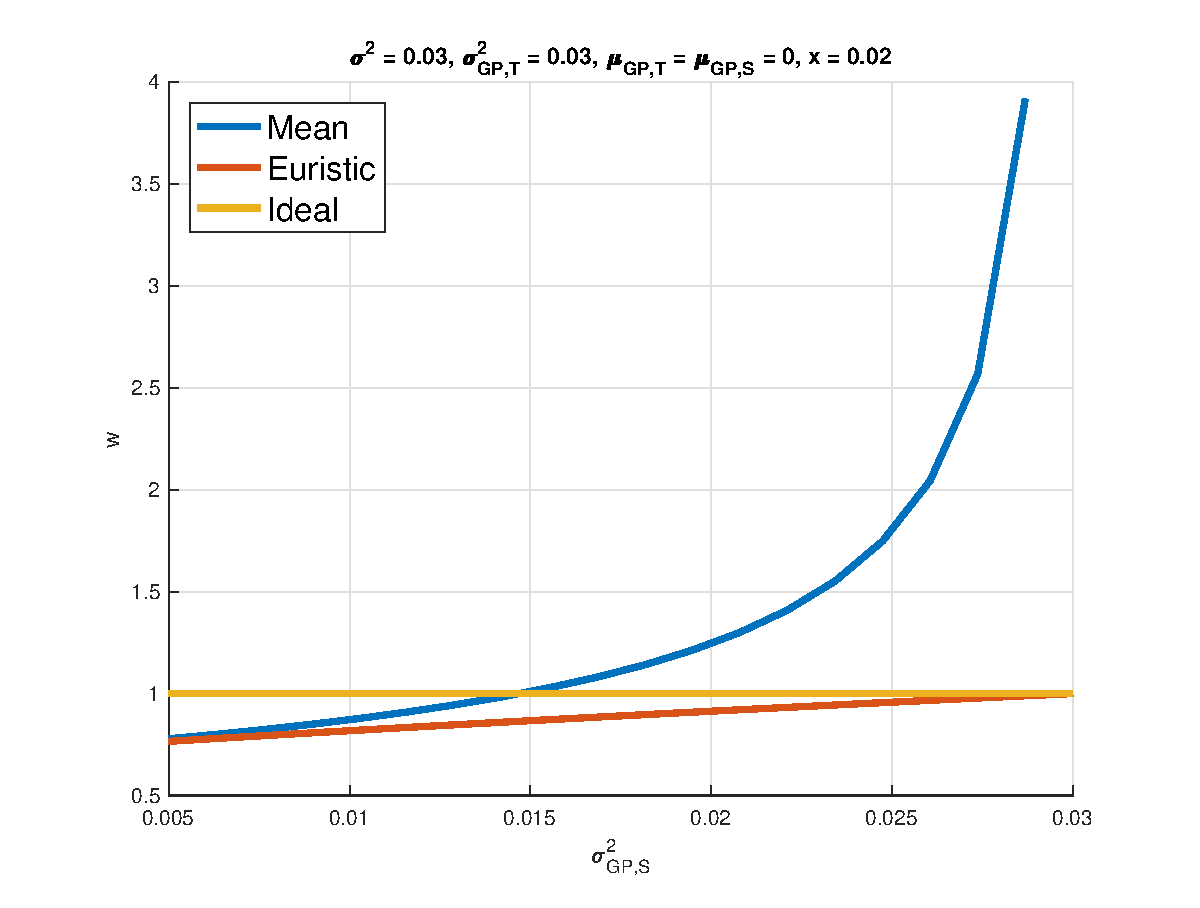
\includegraphics[scale=0.7]{images/weights-plot.eps}
      \caption{Weight estimations according to Equation \ref{mean-weight} (red), \ref{eur} (blue) and the ideal weight (orange)}
      \label{weight-plot}
    \end{figure}

    \noindent A pseudocode implementation of the procedures to estimate weights for rewards and dynamics, in conjunction with
    use \ref{eur}, are given by
    Algorithm \ref{rw_weight_est} and \ref{rw_transition_est}.

    \begin{algorithm}
        \caption{$w_r$ estimation algorithm}\label{rw_weight_est}
        \begin{algorithmic}[1]
          \Procedure{EstimateRwWeight($(s,a,s',r)$, ${GP}_{r}$, $x$)}{}
            \State $W \gets \emptyset$
            \State $\mathcal{N}_{S} = (\mu_{GP,S}, \sigma_{GP,S}^{2}) \gets {GP}^{S}_{r}.predict(s,a)$
            \State $\mathcal{N}_{T} = (\mu_{GP,T}, \sigma_{GP,T}^{2}) \gets {GP}^{T}_{r}.predict(s,a)$
            \For {$i = 0$ $\text{to}$ $N_{samp}$}
              %\State $s_s \gets \mathcal{N}_{s}.sample()$
              %\State $s_t \gets \mathcal{N}_{t}.sample()$
              \State $d_s \gets \mathcal{N}(r; \mu_{GPs}, \sigma^{2}_{r} + \sigma_{GPs}^{2})$
              \State $d_t \gets \mathcal{N}(r; \mu_{GPt}, \sigma^{2}_{r} + \sigma_{GPt}^{2})$
              \State $w_r \gets \frac{d_t}{d_s}$
              \State $W += w_r$
            \EndFor
          \EndProcedure
        \end{algorithmic}
    \end{algorithm}

    \begin{algorithm}
        \caption{$w_p$ estimation algorithm}\label{rw_transition_est}
        \begin{algorithmic}[1]
          \Procedure{EstimateTrWeight($(s,a,s',r)$, ${GP}_{t}$)}{}
            \State $W \gets \emptyset$
            \State $\mathcal{N}_{S} = (\mu_{GP,S}, \sigma_{GP,S}^{2}) \gets {GP}^{S}_{p}.predict(s,a)$
            \State $\mathcal{N}_{T} = (\mu_{GP,T}, \sigma_{GP,T}^{2}) \gets {GP}^{T}_{p}.predict(s,a)$
            \For {$i = 0$ $\text{to}$ $N_{samp}$}
              %\State $s_s \gets \mathcal{N}_{s}.sample()$
              %\State $s_t \gets \mathcal{N}_{t}.sample()$
              \State $d_s \gets \mathcal{N}(s'; \mu_{GPs}, \sigma^{2}_{r} + \sigma_{GPs}^{2})$
              \State $d_t \gets \mathcal{N}(s'; \mu_{GPt}, \sigma^{2}_{r} + \sigma_{GPt}^{2})$
              \State $w_p \gets \frac{d_t}{d_s}$
              \State $W += w_p$
            \EndFor
          \EndProcedure
        \end{algorithmic}
    \end{algorithm}

    \noindent It is also important to notice that the procedure described above is just a possible way to deal with the
    problem of weight estimation. As we will see in the next chapter the learning algorithm (Weighted Fitted Q-Iteration)
    is totally independent of the method used to calculate the weights associated with the sample. This, in our opinion,
    represents a further advantage with respect other transfer learning related algorithms.
